\section{Literature Review}
\quad This chapter surveys the theoretical and technological foundations underpinning our research: variational quantum algorithms, the barren-plateau phenomenon and its causes, existing static and heuristic mitigation strategies, and the use of reinforcement learning in scientific and quantum control problems. We position AL-QNN within this landscape and identify the specific gap it addresses.

\subsection{Overview of the Field}
Quantum machine learning studies how parameterized quantum circuits can represent and learn functions of classical or quantum data. In the variational paradigm, a circuit U($\theta$) prepares a state whose measurement defines a model output; the parameters $\theta$ are optimized classically. The central open problem for these models is trainability, dominated by the barren-plateau phenomenon.

\subsubsection{Variational Quantum Circuits and the Hardware-Efficient Ansatz}
On NISQ hardware, the hardware-efficient ansatz -- alternating layers of single-qubit rotations and fixed entangling gates -- is popular because it respects device connectivity and keeps circuits shallow.

\subsubsection{VQE and VQC: Two Families of Variational Algorithms}
Two broad families of variational algorithm dominate the field. The first, exemplified by the Variational Quantum Eigensolver (VQE), targets physics and chemistry problems where the cost function is the expectation value of a Hamiltonian and the goal is to find its ground-state energy. The second, exemplified by the Variational Quantum Classifier (VQC) used in this project, targets supervised learning problems where the cost function is a classification loss computed from measurement outcomes on labelled data. The two families share the same underlying machinery -- a parameterized circuit, a classical optimizer, and a scalar cost evaluated via measurement -- and, as a consequence, share the same trainability pathology. This is why barren-plateau mitigation strategies developed for VQE chemistry problems, such as ADAPT-VQE, are directly relevant background for a VQC depth-scheduling project even though the target application domains differ.

\subsubsection{Data Encoding Strategies}
A separate but related question is how the classical data enters the circuit in the first place. This project uses angle encoding, where each classical feature is loaded as the rotation angle of a single-qubit gate; this is simple, hardware-efficient, and keeps the encoding circuit shallow, at the cost of requiring one qubit per feature (hence the feature-count-to-qubit-count matching described in Section~4.3). Denser encodings, such as amplitude encoding, can represent exponentially more features per qubit but require circuits that are themselves harder to prepare and differentiate reliably on near-term hardware, which is why angle encoding remains the standard choice for hardware-efficient classifiers of the kind studied here.

\subsection{Historical Context}

\subsubsection{Origins of Variational Quantum Algorithms}
Variational quantum algorithms were introduced with the Variational Quantum Eigensolver of \citet{peruzzo2014variational} and popularized for machine learning by the hardware-efficient ansatz of \citet{kandala2017hardware}.

\subsubsection{Discovery and Refinement of the Barren-Plateau Phenomenon}
The barren-plateau phenomenon was identified by \citet{mcclean2018barren}, who showed that for sufficiently random deep circuits the gradient variance decays exponentially with the qubit count. Subsequent work by \citet{cerezo2021cost} refined this picture, showing that local cost functions exhibit weaker, depth-dependent plateaus, which is precisely the regime this project exploits. Between these two results, the field's understanding of the barren plateau shifted from a qubit-count phenomenon alone to a joint function of qubit count, circuit depth, ansatz expressivity, and the locality of the cost -- a four-factor picture that motivates treating depth as a controllable variable rather than a fixed hyperparameter, which is the starting point for this project's MDP formulation in Section~4.7.2.

\begin{figure}[htbp]
\centering
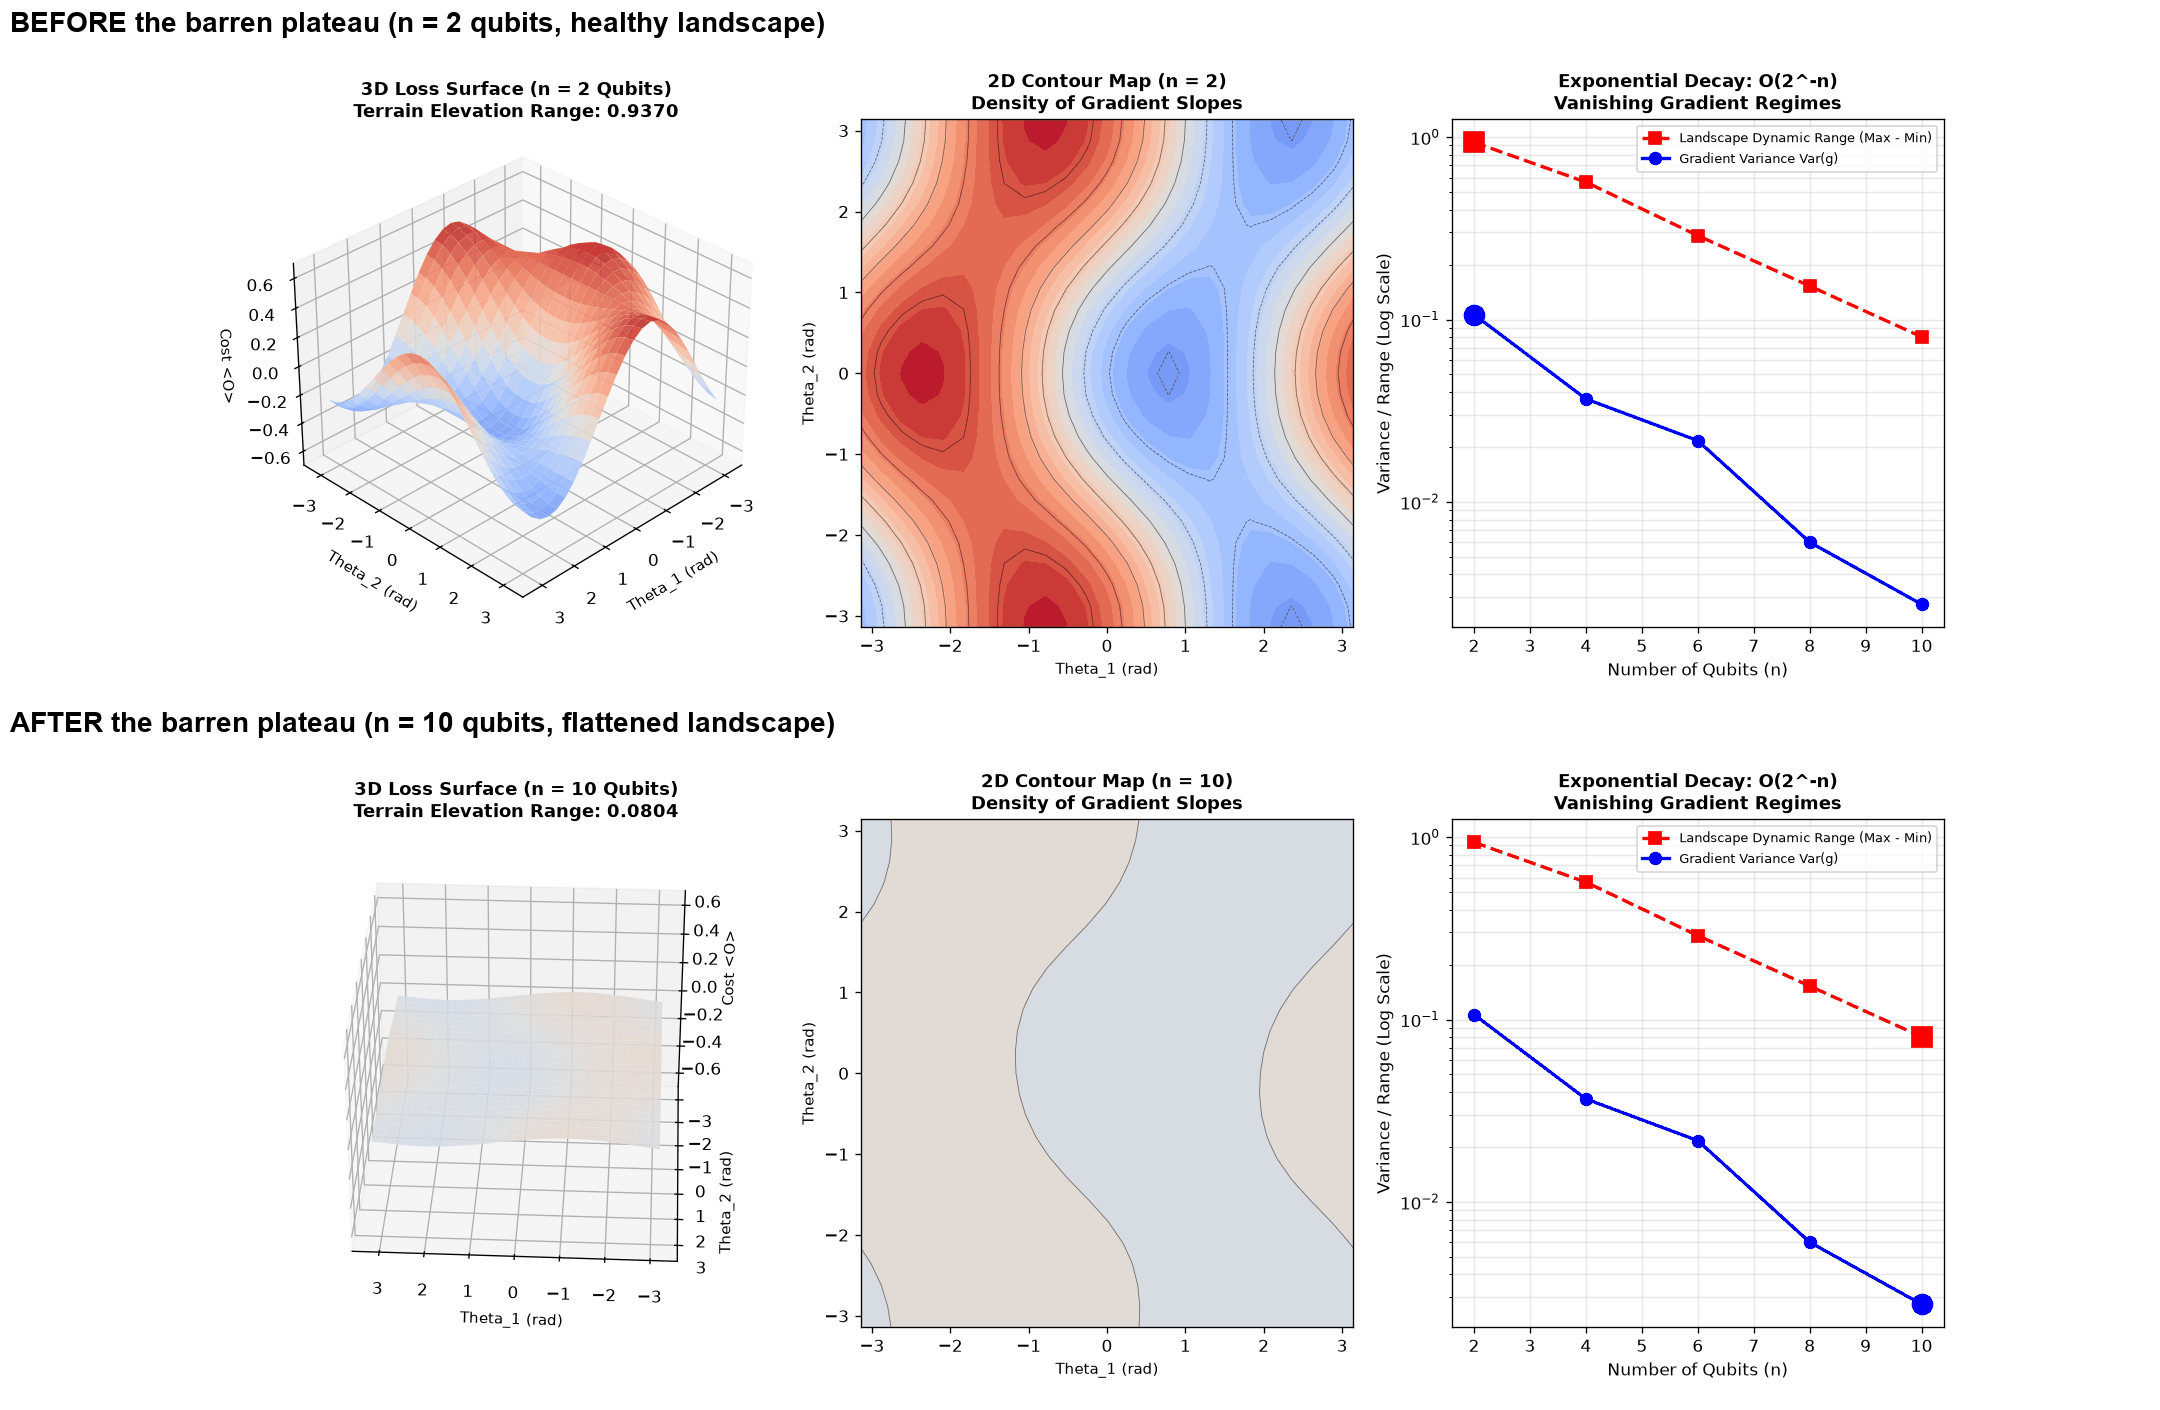
\includegraphics[width=\textwidth]{figure/fig_barren_plateau_theory.png}
\caption{The barren-plateau phenomenon in theory, not an AL-QNN experimental result: the same toy random circuit's cost landscape (left, 3D surface; centre, gradient-slope contour) before the plateau at $n=2$ qubits (top, terrain elevation range 0.937) versus after it at $n=10$ (bottom, range 0.080) -- an $\approx$12$\times$ flattening driven purely by qubit count. The right panel, common to both rows, plots the full $O(2^{-n})$ gradient-variance decay from $n=2$ to $10$, with the marker size highlighting each row's qubit count. This illustrates \citet{mcclean2018barren}'s general result and is independent of the project's own $n\le8$ evaluation scope (Section~1.6, Section~6.1).}
\label{fig:bp_theory}
\end{figure}

\subsection{Causes of Barren Plateaus}
The literature identifies several, partially overlapping, mechanisms that produce barren plateaus, and it is worth distinguishing them because they call for different mitigations.

\subsubsection{Expressivity-Induced Plateaus}
The mechanism formalized by \citet{mcclean2018barren} arises when the ansatz is expressive enough to approximate a 2-design, so that the parameter landscape looks locally random almost everywhere and the gradient variance collapses exponentially with qubit count regardless of what is being optimized. \citet{du2020expressive} formalize this expressivity itself via the circuit's covering number, giving a quantitative basis for the same expressivity-trainability trade-off that motivates treating depth -- not just qubit count -- as a lever on how expressive, and therefore how plateau-prone, the ansatz becomes.

\subsubsection{Cost-Function-Induced Plateaus}
The mechanism refined by \citet{cerezo2021cost} arises separately from how the cost is measured: a global cost that reads out correlations across the whole register concentrates exponentially in the qubit count even for shallow circuits, whereas a local cost that reads out a small, fixed-size subset of qubits only concentrates once the circuit is deep enough for that subset to become entangled with the rest of the system -- which is the origin of the depth-dependent slope measured empirically in Section~6.1.

\subsubsection{Noise-Induced Plateaus and Scope of This Project}
A third, noise-induced mechanism, documented elsewhere in the literature, arises on real hardware from decoherence and gate errors compounding with circuit depth; because this project runs on a noiseless statevector simulator (Section~1.6), noise-induced plateaus are explicitly out of scope, and every plateau observed and mitigated in this report is of the expressivity- or cost-induced kind.

\subsubsection{Relevance to Scheduler Design}
This distinction matters directly for the scheduler design: because the local-cost, depth-dependent plateau is the one this project targets, the reward system (Section~4.7.3) and the recommendation to prefer a local cost (Section~6.4) both follow from \citet{cerezo2021cost}'s result specifically, not from barren-plateau theory in general.

\subsection{Static and Heuristic Mitigation Strategies}
Existing mitigation strategies for barren plateaus fall into three broad categories, each of which informs one part of the baseline comparison in Section~6.

\subsubsection{Structured Initialization}
\citet{grant2019initialization} show that initializing parameters so that the circuit starts close to the identity -- rather than at a uniformly random point -- avoids the plateau at the start of training even for expressive ansätze, because the initial landscape is not yet random. This is a one-time, static intervention: it changes where training starts, not how the architecture evolves during training, which is the gap this project addresses.

\subsubsection{Layerwise Learning}
Related grow-then-freeze heuristics train a circuit one layer at a time, freezing already-trained layers before adding the next. This is conceptually the closest prior approach to AL-QNN's depth scheduling, since both grow the circuit progressively; the difference is that layerwise learning grows on a fixed, pre-determined schedule, while AL-QNN's agent decides whether and when to grow based on live telemetry, and can also prune or freeze growth entirely.

\subsubsection{Adaptive Operator Construction (ADAPT-VQE)}
\citet{grimsley2019adaptive} (ADAPT-VQE) grow an ansatz operator-by-operator, greedily selecting at each step the operator with the largest gradient. This is adaptive in the sense that the final circuit structure is not fixed in advance, but the selection rule itself is a fixed, hand-designed greedy heuristic -- exactly the kind of static policy that AL-QNN's greedy baseline (\Cref{tab:ai4i,tab:heart,tab:sim8g}) formalizes and directly compares against a learned alternative.

\subsection{Reinforcement Learning in Scientific and Quantum Applications}

\subsubsection{RL for Scientific Control Problems}
Reinforcement learning has been applied to a growing range of scientific control problems where the environment is expensive to evaluate and the optimal policy is not known in closed form -- from robotic control to, more recently, quantum circuit design and pulse-level control. A recurring theme in this literature is that the environment's cost of evaluation, not the learning algorithm, is usually the binding constraint: a physical or high-fidelity simulated environment can be too slow to supply the millions of interactions that modern deep RL methods need. This is exactly the constraint that shapes AL-QNN's two-simulator design (Section~4.7.1) -- training against a fast, calibrated surrogate and only deploying the learned policy against the expensive, physically faithful PennyLane backend is the same train-cheap-deploy-faithful pattern behind domain randomization and sim-to-real transfer in robotics \citep{tobin2017domain}, applied here to make training tractable without abandoning a faithful evaluation step.

\subsubsection{Design Philosophy: Off-the-Shelf Algorithms, Domain-Specific MDP}
The two algorithms used in this project, PPO \citep{schulman2017proximal} and DQN \citep{mnih2015human}, are general-purpose deep RL methods with no quantum-specific modification, which is a deliberate design choice: the project's contribution is in how the MDP is constructed around the circuit (Section~4.7), not in a novel RL algorithm. The two were chosen because they represent complementary points in the design space, and neither is assumed a priori to be the better fit for a quantum-telemetry MDP. PPO is on-policy and update-conservative (its clipped objective bounds how far a single update can move the policy), which tends to make training stable but requires fresh interaction data at every update. DQN is off-policy and reuses past interactions through a replay buffer, which can be more sample-efficient but is also more prone to instability when combined with function approximation over a continuous-valued telemetry state. Running both against the identical state, action space, and reward lets Section~6 attribute any performance gap to this stability/sample-efficiency trade-off rather than to an arbitrary choice of algorithm. This mirrors the broader trend in scientific RL applications, where the engineering effort typically goes into designing an informative state and reward from domain telemetry, while the learning algorithm itself is taken off the shelf.

\subsection{Technological Advancements}
Two practical advances make this project feasible.

\subsubsection{Differentiable Quantum Simulation (PennyLane)}
Differentiable quantum-simulation libraries such as PennyLane \citep{bergholm2018pennylane} allow exact statevector gradients via backpropagation, so gradient telemetry can be measured directly. This matters because the standard way to obtain a gradient from a real quantum device -- the parameter-shift rule -- requires evaluating the circuit twice per parameter on hardware, which is affordable for a handful of gradient checks but far too slow to supply the per-epoch gradient-variance telemetry (Section~4.7.2) that the scheduler's state depends on. A statevector simulator sidesteps this entirely: because the full quantum state is available in memory, backpropagation computes every parameter's gradient in a single reverse pass, the same way it would for a classical neural network. This is what makes it computationally realistic to log gradient variance, gradient norm, and the near-zero-gradient ratio at every epoch of every run, rather than only at a few checkpoints.

\subsubsection{Mature Deep Reinforcement Learning Algorithms}
Mature deep reinforcement-learning algorithms -- PPO \citep{schulman2017proximal} and DQN \citep{mnih2015human} -- provide stable policy optimization that can be pointed at the depth-scheduling problem once it is framed as an MDP. Both ship in well-tested open-source implementations with established default hyperparameters, which removes algorithm-level tuning as a variable and lets the experimental effort concentrate on the parts of the system that are specific to this project: the sixteen-dimensional telemetry state, the five-action mutation interface, and the reward weights of \Cref{tab:reward}.

\subsection{Related Work and Research Gaps}

\subsubsection{Comparison of Existing Systems}
\begin{table}[htbp]
\centering
\caption{Comparison of depth-control approaches.}
\label{tab:comparison}
\begin{tabular}{|p{3cm}|p{3.5cm}|p{2.7cm}|p{2.8cm}|}
\hline
\textbf{Approach} & \textbf{Depth control} & \textbf{Uses live telemetry?} & \textbf{Learned?} \\
\hline
Fixed-depth HEA & Manual, fixed & No & No \\
Layerwise learning & Grow-then-freeze, heuristic & Partial & No \\
ADAPT-VQE & Operator growth by gradient & Yes (gradient) & No (greedy) \\
AL-QNN (this work) & Online add/prune of layers & Yes (16-dim telemetry) & Yes (PPO/DQN) \\
\hline
\end{tabular}
\end{table}

\subsubsection{Gaps in the Literature and Justification for the Project}
Existing mitigation strategies are largely static or greedy: they either fix the depth, grow it by a fixed schedule, or add operators one at a time by immediate gradient magnitude. None of them frame depth control as a sequential decision problem in which an agent learns a policy over rich circuit telemetry, and none provide an honest, multi-regime characterization of when such adaptation actually helps versus when a simple rule suffices. This is the gap AL-QNN addresses.

Concretely, each strategy reviewed in Section~3.4 leaves a specific gap that motivates one part of AL-QNN's design. Structured initialization \citep{grant2019initialization} intervenes only once, before training starts, and has nothing to say about how the architecture should evolve once training is underway -- AL-QNN instead makes depth a variable the agent can revisit at every epoch. Layerwise learning grows on a schedule fixed in advance, independent of whether the circuit's gradients are actually healthy at the moment of growth -- AL-QNN conditions every growth decision on the live sixteen-dimensional telemetry state, so a layer is added only when the observed evidence supports it. ADAPT-VQE \citep{grimsley2019adaptive} does use live gradient information, but its selection rule is a fixed, hand-designed greedy heuristic (always add the operator with the largest instantaneous gradient); AL-QNN instead learns the mapping from telemetry to action end-to-end via PPO and DQN, allowing the policy to weigh gradient health against loss trajectory and resource cost jointly, rather than by a single hard-coded criterion. \Cref{tab:comparison} summarizes this progression from manual, to scheduled, to greedy-adaptive, to learned-adaptive depth control.

None of these three prior strategies, nor the reinforcement-learning applications surveyed in Section~3.5, report results across multiple cost-type regimes with an explicit accounting of where the approach fails. This project's empirical contribution is therefore not only the learned scheduler itself, but the multi-regime evaluation of Section~6, which is designed specifically to expose the boundary between the regime where adaptive scheduling helps and the regime where it does not -- a boundary that the reviewed literature does not characterize because none of the reviewed methods are evaluated against a matched static baseline across more than one regime.
